\subsection{Spherical Collapse (ex 4)}

To validate the numerical implementation of the spherical collapse solver, two primary tests were performed: (i) verifying the equivalence among formulations A, B, and C under non-linear integration, and (ii) determining the linear collapse threshold $\delta_c(z)$ using a bisection shooting method across different cosmological models.

\subsubsection{Equivalence of Formulations A, B, C}

To assess the numerical equivalence among the three spherical collapse formulations (Models A, B, and C), each model was integrated from an initial scale factor $a_i = 10^{-4}$ ($\delta_i = 10^{-4}$) to $a_f = 1.0$ within a fiducial flat $\Lambda\mathrm{CDM}$ background ($\Omega_{m,0} = 0.315$). 
Table~\ref{tab:sc_equivalence} summarizes the final density contrast $\delta(a_f)$ and the maximum relative differences evaluated with respect to Model A. Models B and C reproduce the reference Model A trajectory with maximum relative differences bounded at $5.52 \times 10^{-9}$ and $5.79 \times 10^{-7}$, respectively, demonstrating high numerical agreement across the formulations.
    \begin{table}[htbp]
        \centering
        \caption{Numerical comparison and relative errors among Spherical Collapse Models A, B, and C integrated from $a_i = 10^{-4}$ ($\delta_i = 10^{-4}$) to $a_f = 1.0$ in flat $\Lambda$CDM ($\Omega_{m,0} = 0.315$).}
        \label{tab:sc_equivalence}
        \begin{tabular}{lcccc}
            \hline
            \textbf{Model} & $\delta(a_i)$ & $\delta(a_f)$ & \textbf{Max. Rel. Diff. vs. Model A} \\
            \hline
            Model A ($\delta, \delta_N$) & $1.000000 \times 10^{-4}$ & $1.939895$ & Reference \\
            Model B ($\delta, \theta$)   & $1.000000 \times 10^{-4}$ & $1.939895$ & $5.5159 \times 10^{-9}$ \\
            Model C ($g, \theta$)        & $1.000000 \times 10^{-4}$ & $1.939894$ & $5.7892 \times 10^{-7}$ \\
            \hline
        \end{tabular}
    \end{table}

Figure~\ref{fig:sc_models_evolution} displays the scale factor evolution of the overdensity $\delta(a)$ and the velocity divergence $\theta(a) \equiv \nabla \cdot \mathbf{v} / (a H)$. The trajectories across Models A, B, and C exhibit complete numerical overlap throughout the entire non-linear evolution up to $a = 1.0$.
    \begin{figure}[H]
        \centering
        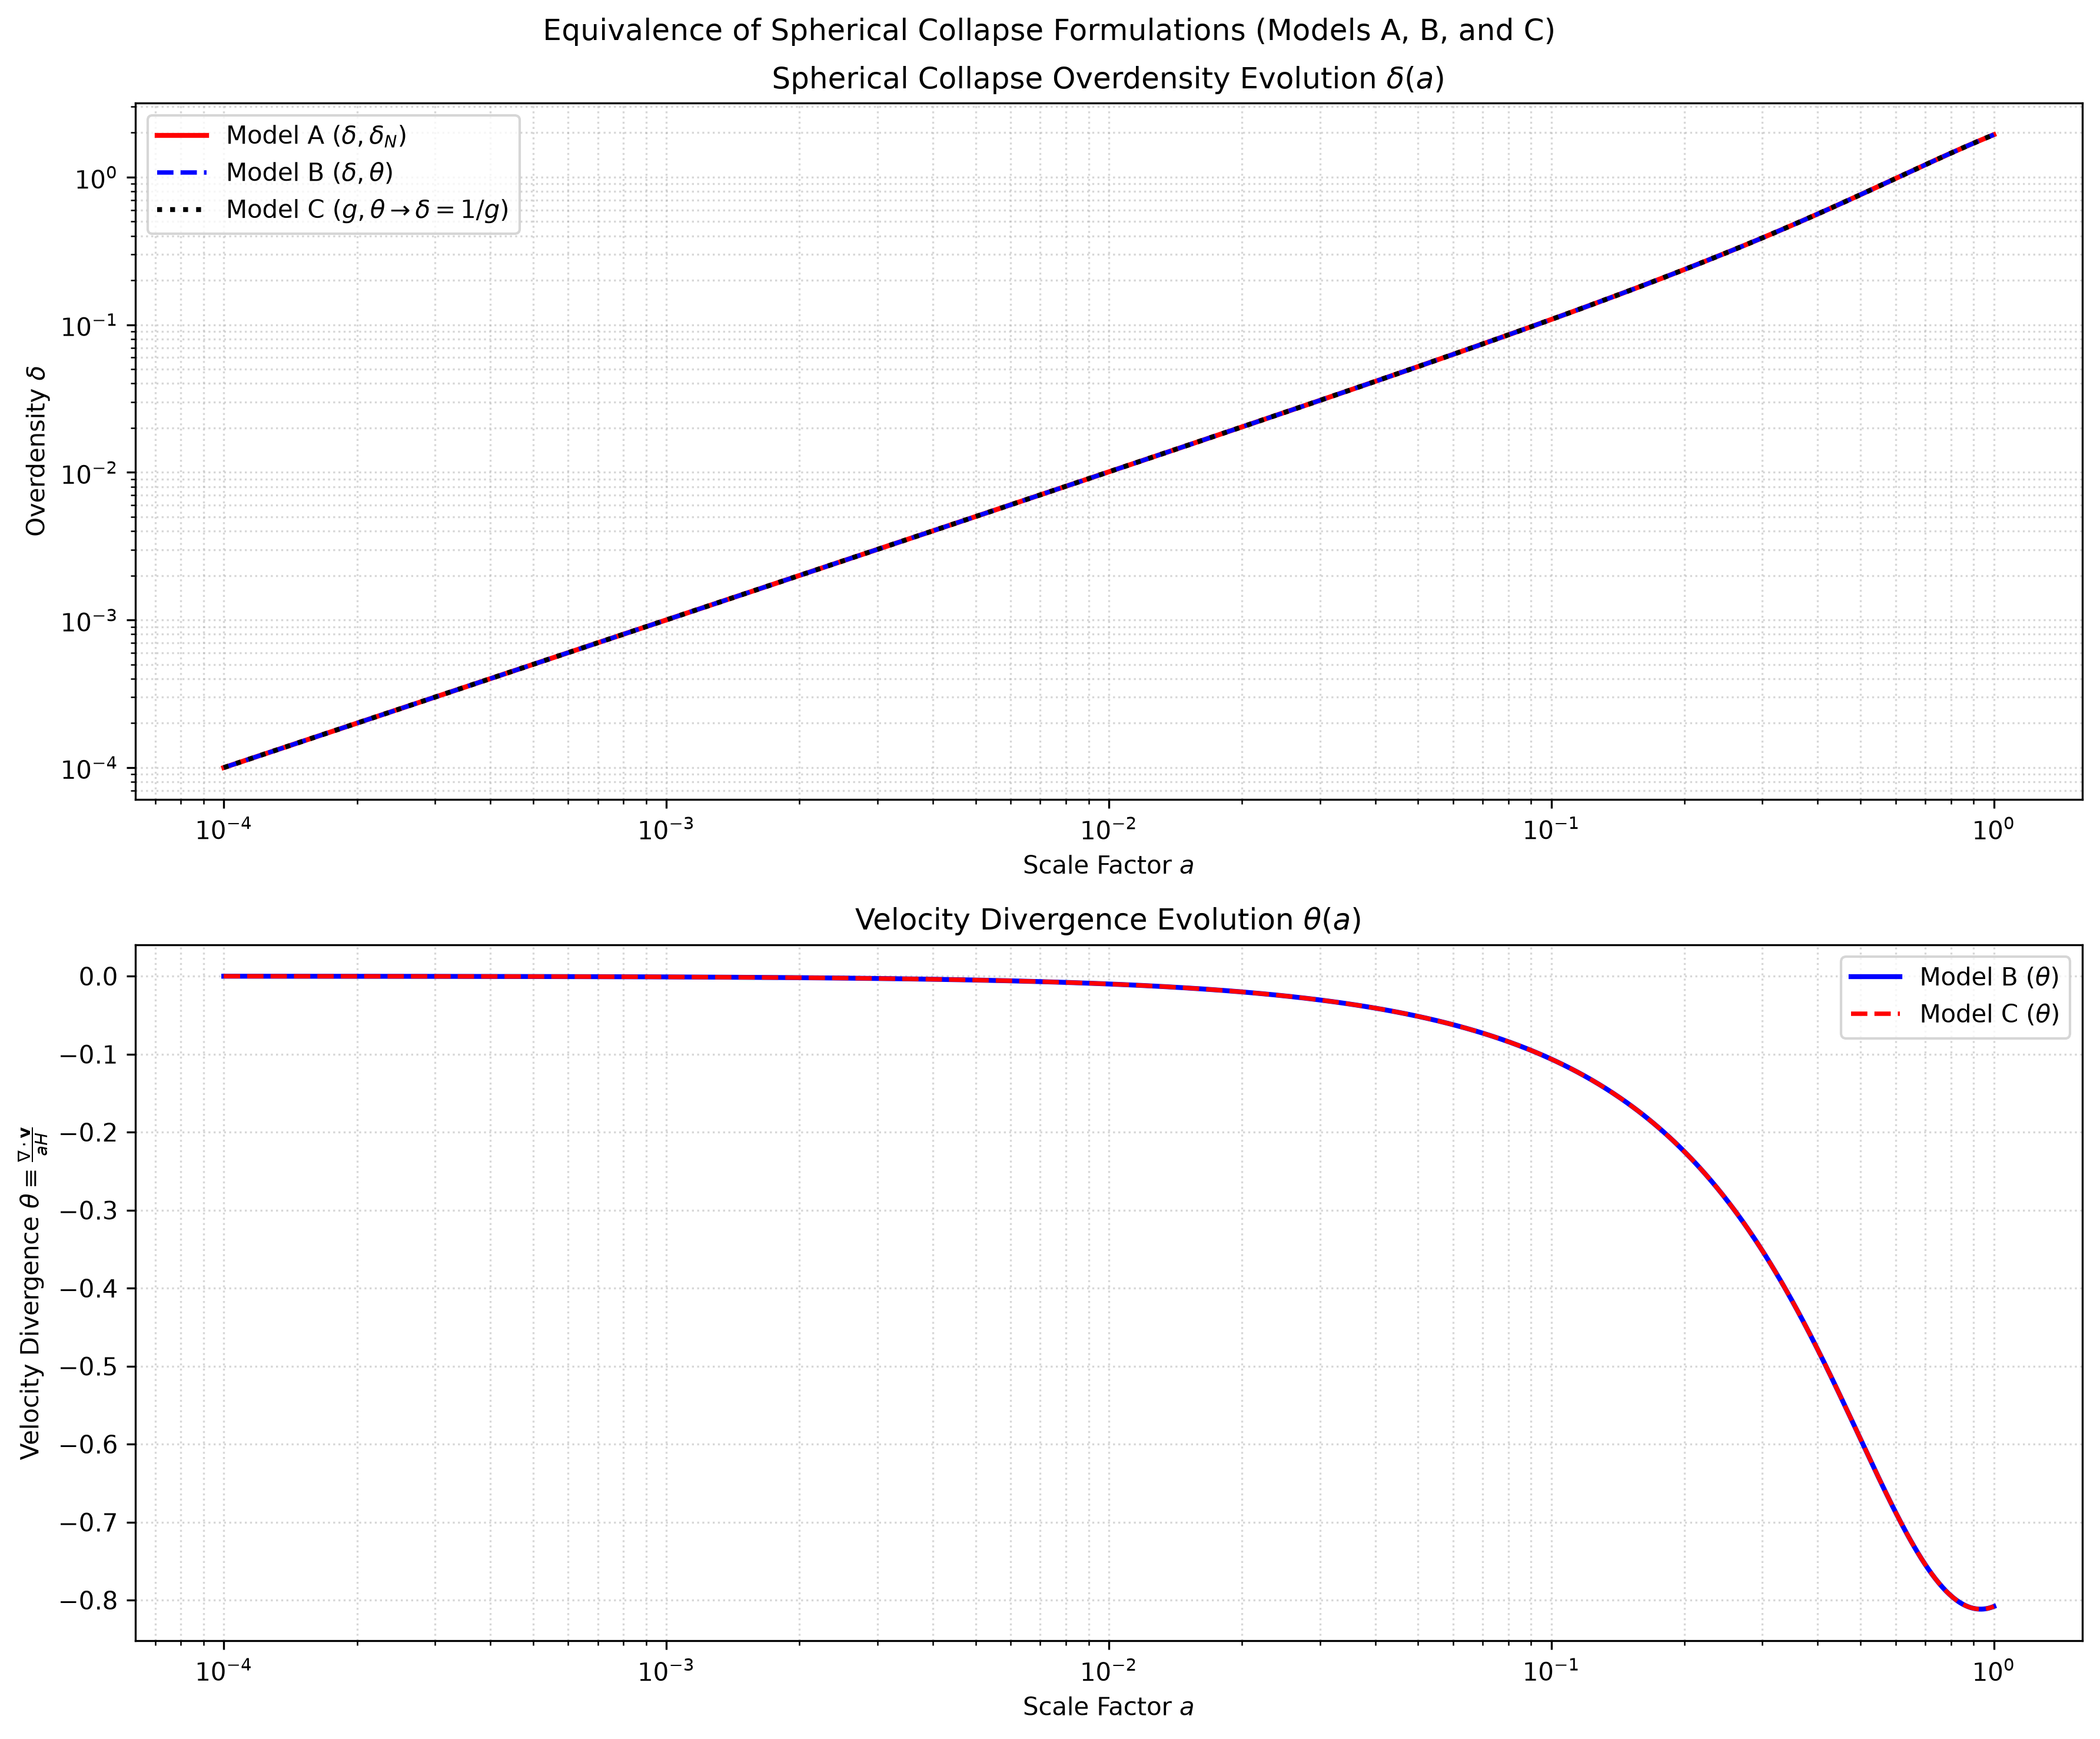
\includegraphics[width=0.8\textwidth]{Figures/Test_20261014_174525_spherical_collapse_models.png}
        \caption{Evolution of the overdensity $\delta(a)$ (top) and velocity divergence $\theta(a)$ (bottom) for Models A, B, and C integrated from $a_i = 10^{-4}$ to $a_f = 1.0$, demonstrating complete numerical overlap.}
        \label{fig:sc_models_evolution}
    \end{figure}
    
\subsubsection{Linear Collapse Threshold \texorpdfstring{$\delta_c(z)$}{delta	textunderscore c(z)} and Shooting Method Validation}

    \begin{figure}[H]
        \centering
        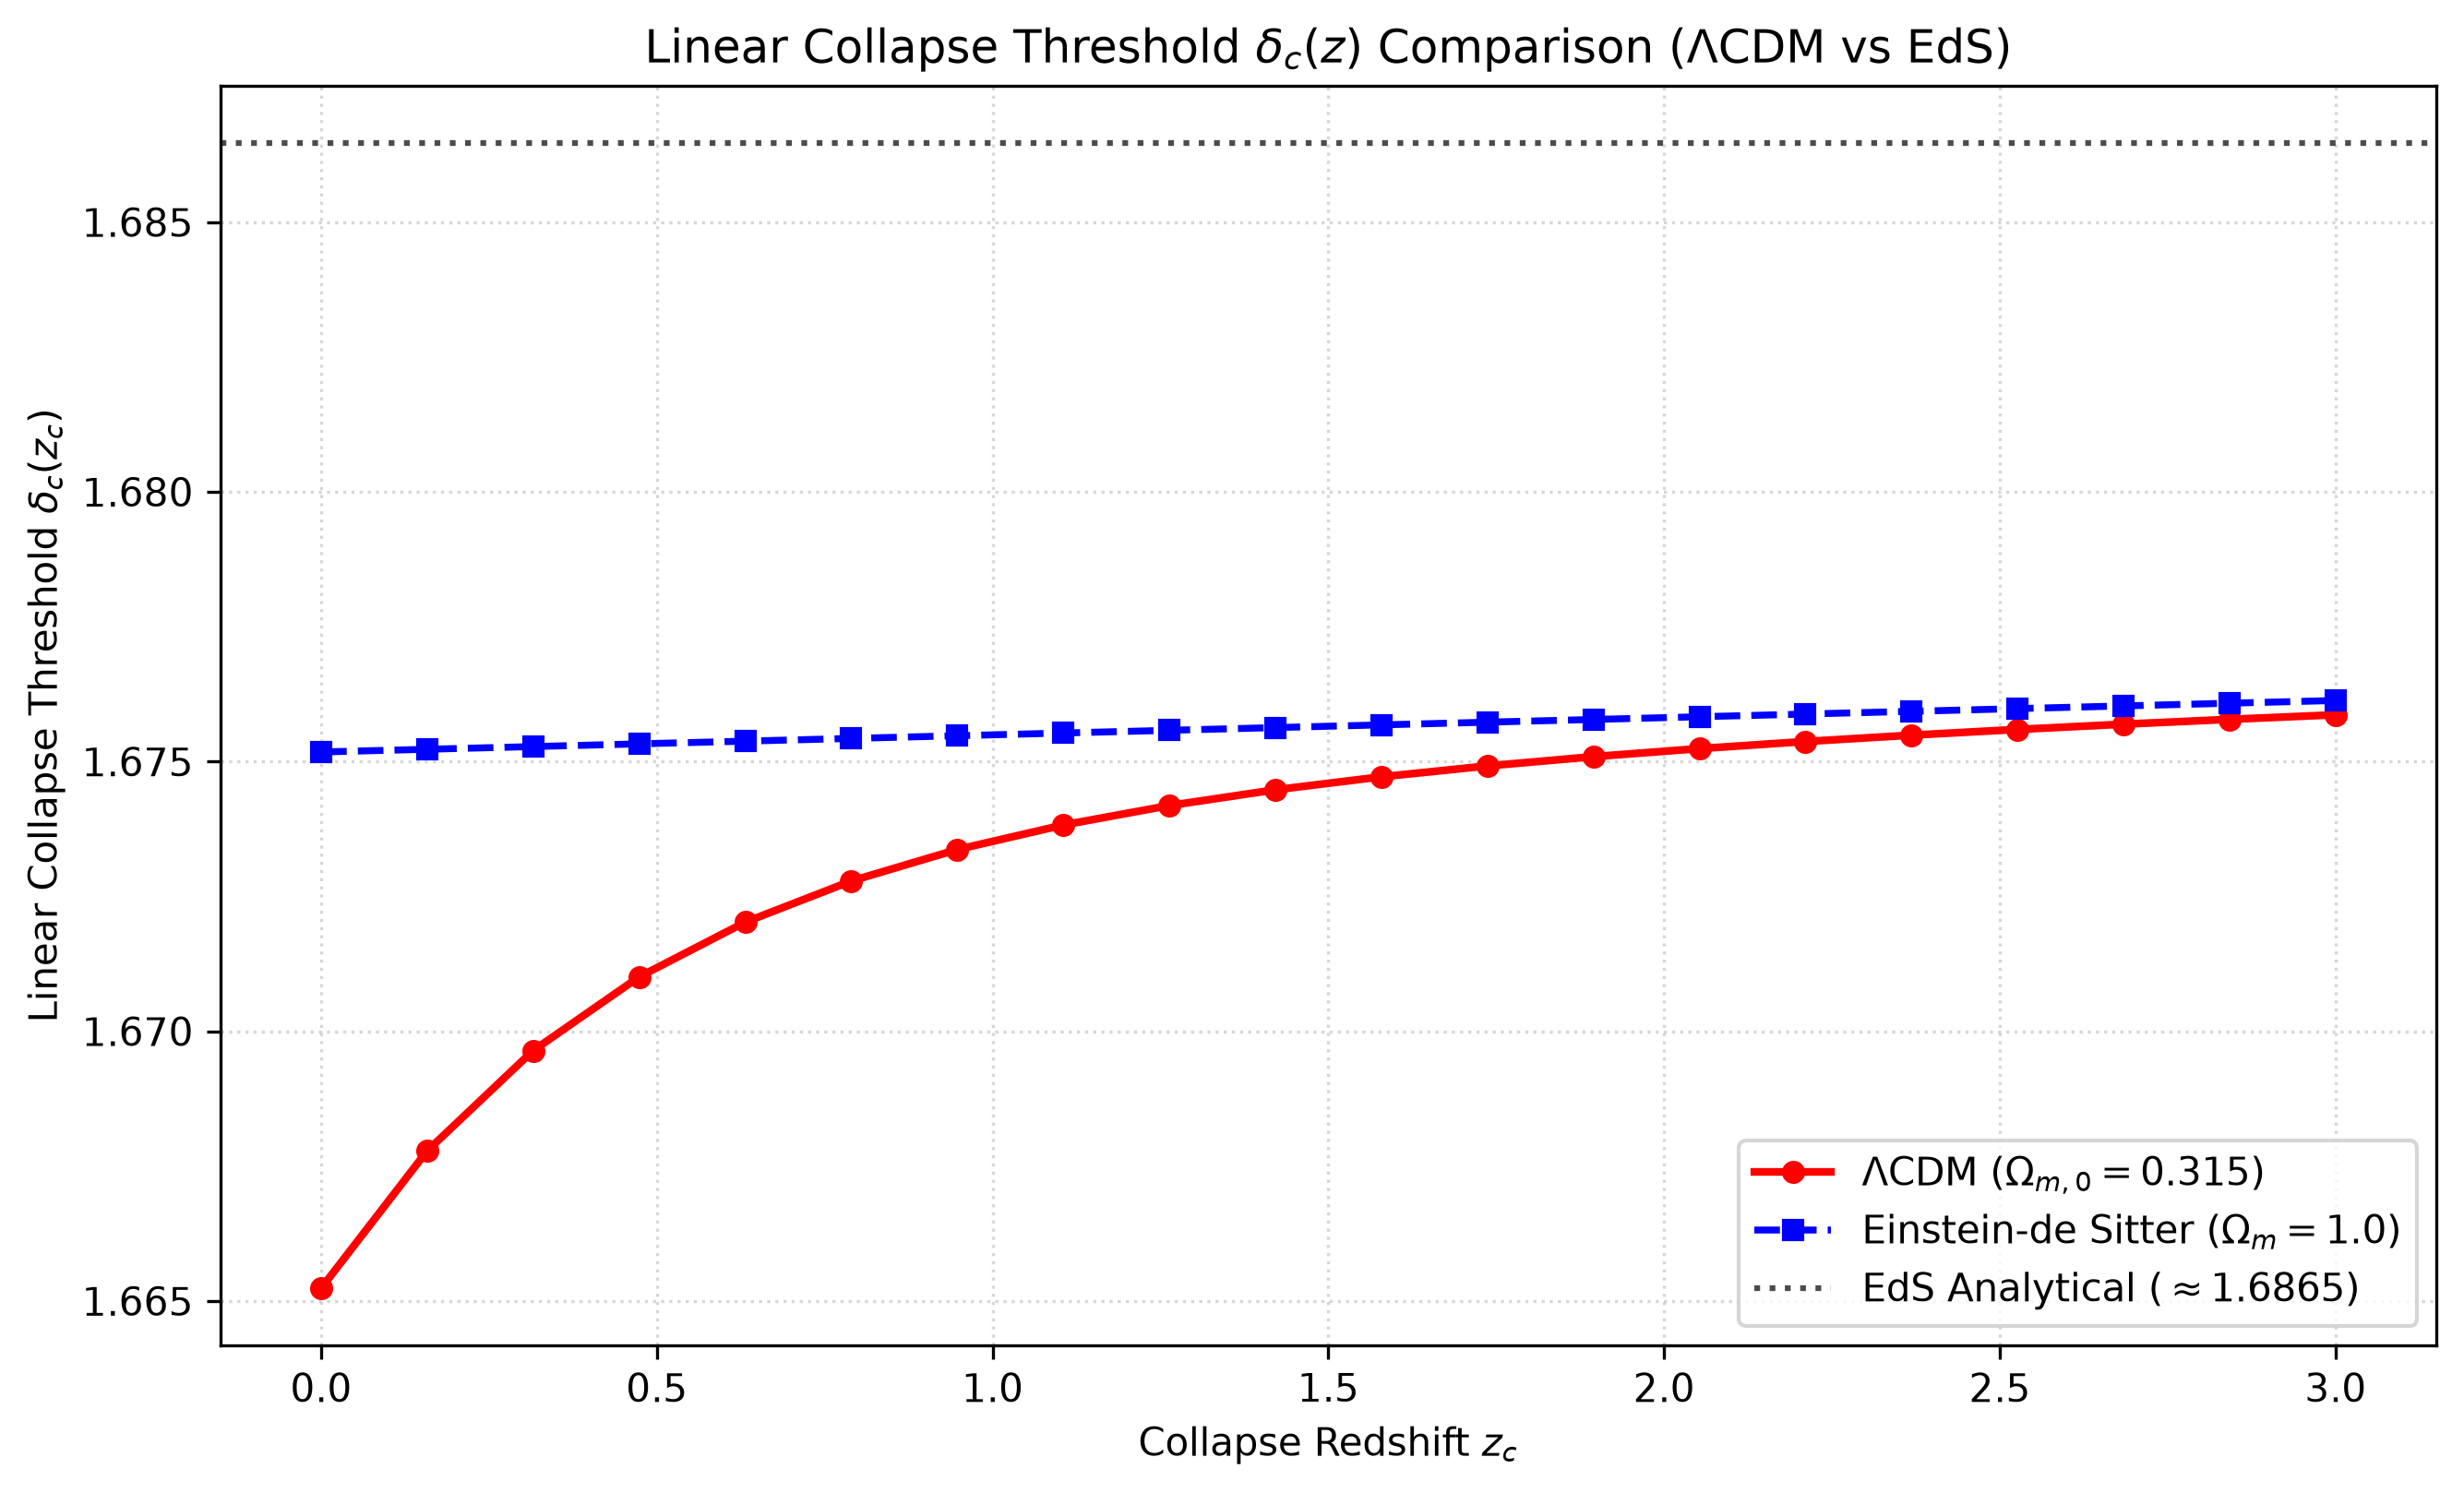
\includegraphics[width=0.8\textwidth]{Figures/Test_20261014_174525_delta_c_redshift_evolution.png}
        \caption{Linear collapse threshold $\delta_c(z_c)$ as a function of collapse redshift $z_c$ comparing flat $\Lambda$CDM ($\Omega_{m,0}=0.315$) and Einstein--de Sitter ($\Omega_m=1.0$).}
        \label{fig:deltac_redshift}
    \end{figure}
    
The critical linear collapse threshold $\delta_c(z_c)$ was determined using a bisection shooting algorithm designed to tune the initial amplitude $\delta_i$ at $a_i$ such that the non-linear perturbation reaches formal collapse at target redshift $z_c$.
Figure~\ref{fig:deltac_redshift} illustrates the redshift evolution of $\delta_c(z_c)$ in flat $\Lambda\mathrm{CDM}$ ($\Omega_{m,0} = 0.315$) compared against the Einstein--de Sitter ($\Omega_m = 1.0$) benchmark and its analytical limit ($\delta_c \approx 1.6865$). While the EdS threshold remains nearly constant near $1.675 \to 1.6765$, dark energy domination at late times ($z_c \to 0$) in $\Lambda\mathrm{CDM}$ suppresses linear growth relative to the non-linear evolution, lowering the threshold to $\delta_c(0) = 1.665235$.

To verify that the shooting algorithm delivers formulation-independent results, $\delta_c(z_c)$ was evaluated across discrete collapse redshifts $z_c \in \{0.0, 0.5, 1.0, 2.0, 3.0\}$ for Models A, B, and C. As detailed in Table~\ref{tab:collapse_statistics_0315}:

 \begin{table}[H]
\centering
\small

% (a) Initial density contrast
\textbf{(a) Mean initial density contrast $\delta_i$}
\label{tab:delta_c_models_comparison}
\begin{tabular}{c ccc}
\toprule
$z_c$ & Model A & Model B & Model C \\
\midrule
0.0 & $7.882788\times10^{-4}$ & $7.882788\times10^{-4}$ & $7.882788\times10^{-4}$ \\
0.5 & $1.029585\times10^{-3}$ & $1.029585\times10^{-3}$ & $1.029585\times10^{-3}$ \\
1.0 & $1.307543\times10^{-3}$ & $1.307543\times10^{-3}$ & $1.307543\times10^{-3}$ \\
1.5 & $1.602818\times10^{-3}$ & $1.602818\times10^{-3}$ & $1.602818\times10^{-3}$ \\
2.0 & $1.906652\times10^{-3}$ & $1.906652\times10^{-3}$ & $1.906652\times10^{-3}$ \\
2.5 & $2.215173\times10^{-3}$ & $2.215172\times10^{-3}$ & $2.215173\times10^{-3}$ \\
3.0 & $2.526552\times10^{-3}$ & $2.526552\times10^{-3}$ & $2.526552\times10^{-3}$ \\
\bottomrule
\end{tabular}

\vspace{0.4cm}

% (b) Critical collapse threshold
\textbf{(b) Critical linear collapse threshold $\delta_c(z_c)$}

\begin{tabular}{c ccc}
\toprule
$z_c$ & Model A & Model B & Model C \\
\midrule
0.0 & 1.67624 & 1.67624 & 1.67624 \\
0.5 & 1.68279 & 1.68279 & 1.68279 \\
1.0 & 1.68560 & 1.68560 & 1.68560 \\
1.5 & 1.68712 & 1.68712 & 1.68712 \\
2.0 & 1.68815 & 1.68815 & 1.68815 \\
2.5 & 1.68898 & 1.68898 & 1.68898 \\
3.0 & 1.68971 & 1.68971 & 1.68971 \\
\bottomrule
\end{tabular}

\vspace{0.4cm}

% (c) Numerical standard deviation
\textbf{(c) Numerical standard deviation}

\begin{tabular}{c ccc}
\toprule
$z_c$ & Model A & Model B & Model C \\
\midrule
0.0 & $2.2637\times10^{-3}$ & $2.2637\times10^{-3}$ & $2.2637\times10^{-3}$ \\
0.5 & $2.7602\times10^{-3}$ & $2.7602\times10^{-3}$ & $2.7602\times10^{-3}$ \\
1.0 & $3.3459\times10^{-3}$ & $3.3459\times10^{-3}$ & $3.3459\times10^{-3}$ \\
1.5 & $3.9863\times10^{-3}$ & $3.9863\times10^{-3}$ & $3.9863\times10^{-3}$ \\
2.0 & $4.6586\times10^{-3}$ & $4.6586\times10^{-3}$ & $4.6586\times10^{-3}$ \\
2.5 & $5.3506\times10^{-3}$ & $5.3506\times10^{-3}$ & $5.3506\times10^{-3}$ \\
3.0 & $6.0555\times10^{-3}$ & $6.0555\times10^{-3}$ & $6.0555\times10^{-3}$ \\
\bottomrule
\end{tabular}

\caption{
Mean initial density contrast, critical linear collapse threshold,
and numerical standard deviation for Models A, B, and C,
considering $\Omega_{m,0}=0.315$.
}
\label{tab:collapse_statistics_0315}

\end{table}

This cross-model consistency is illustrated in Figure~\ref{fig:models_deltac_comparison}, where the threshold curves for Models A, B, and C overlap across the entire evaluated redshift range.
    \begin{figure}[H]
        \centering
        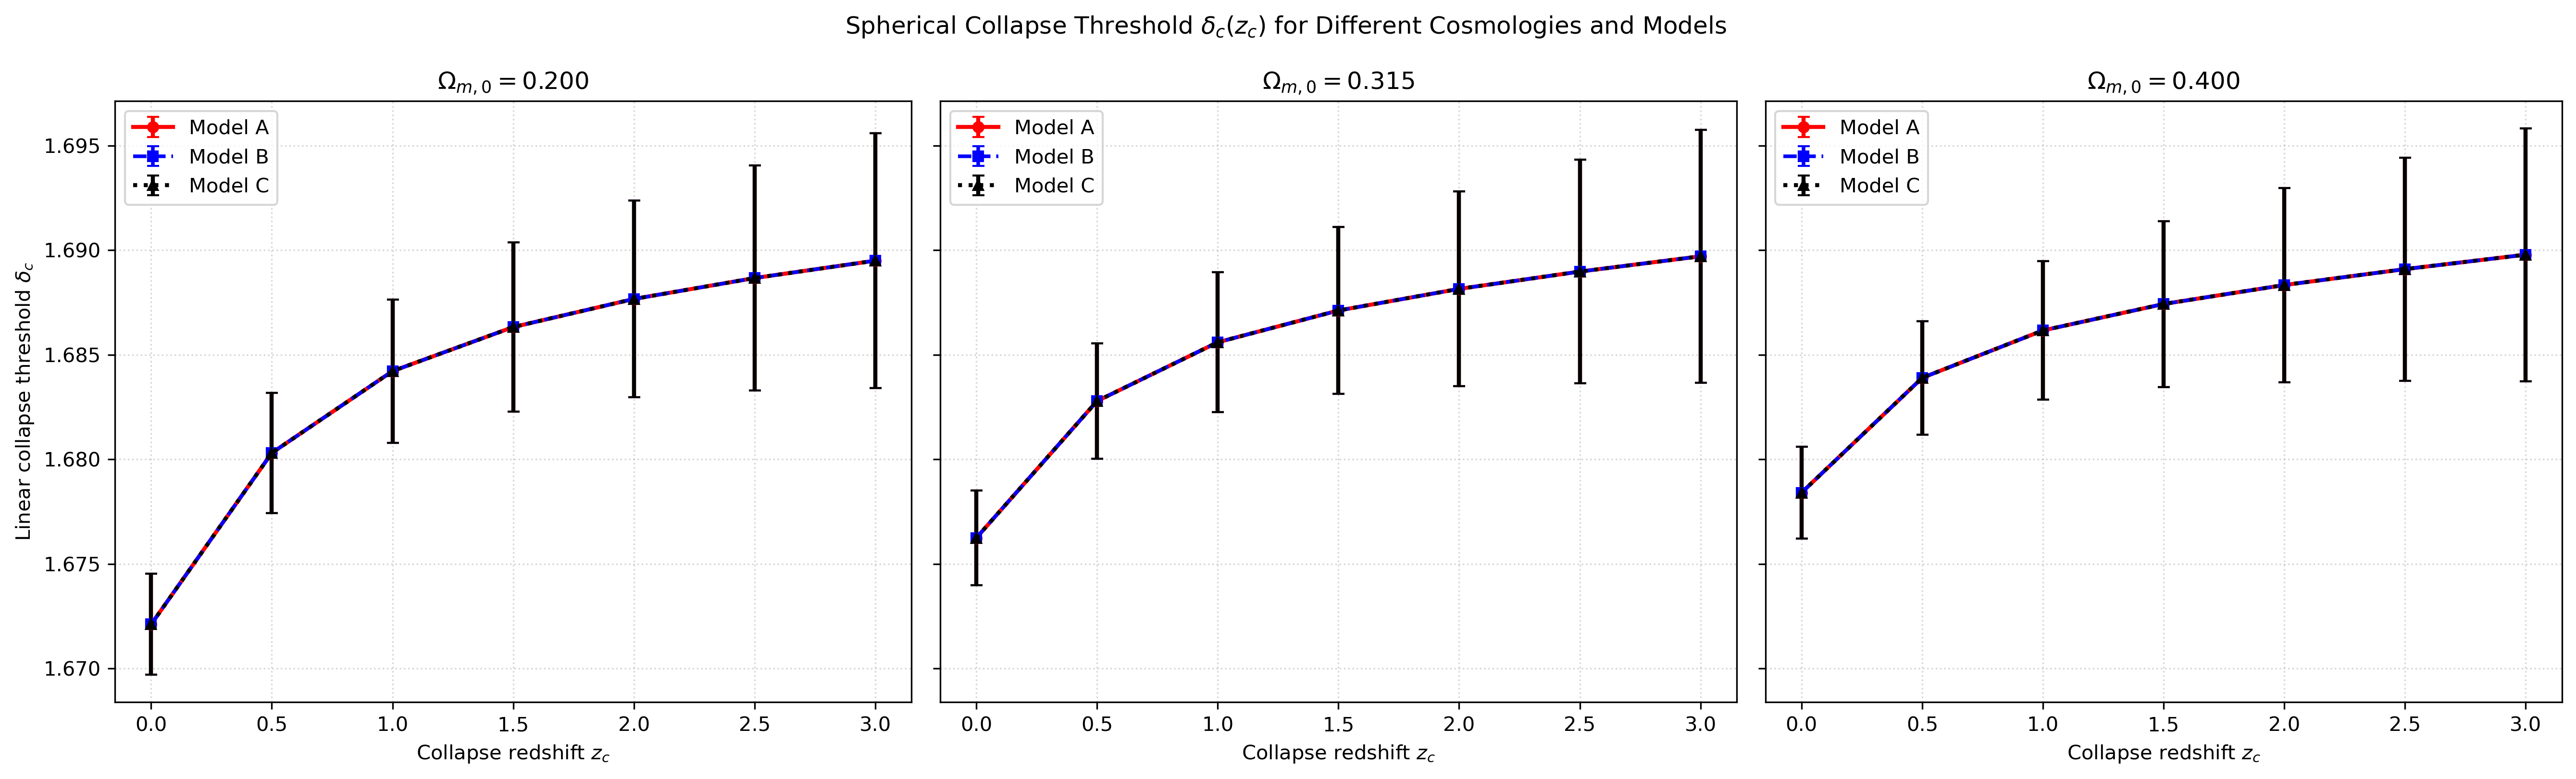
\includegraphics[width=0.85\textwidth]{Figures/Test_20261014_174525_models_delta_c_comparison.png}
        \caption{Linear collapse threshold $\delta_c(z_c)$ calculated across discrete redshifts $z_c \in \{0, 0.5, 1, 2, 3\}$ for Models A, B, and C, confirming cross-model consistency.}
        \label{fig:models_deltac_comparison}
    \end{figure}

\subsubsection{Cosmological Grid Analysis and Independent Audit}

To systematically map spherical collapse observables, a cosmological grid comprising three models (A, B, and C), seven collapse redshifts, $z_c \in \{0, 0.5, 1.0, 1.5, 2.0, 2.5, 3.0\}$, and three matter densities, $\Omega_{m,0} \in \{0.2, 0.315, 0.4\}$, was computed.

An independent mathematical audit confirmed the precision of all turnaround and virial observables
\begin{itemize}

    \item The turnaround event condition $\theta_{\mathrm{ta}} + 3 = 0$ was located with residuals bounded below $5.3291 \times 10^{-15}$.

    \item The matter-referenced virial overdensity $\Delta_{\mathrm{vir,m}}$ formula error was bounded below $4.5475 \times 10^{-13}$.

    \item The critical-referenced virial overdensity $\Delta_{\mathrm{vir,c}}$ formula error was bounded below $3.9790 \times 10^{-13}$.

    \item The cubic virial polynomial residual $4\lambda_{\mathrm{ta}}y_{\mathrm{vir}}^3 - 2(1+\lambda_{\mathrm{ta}})y_{\mathrm{vir}} + 1 = 0$ yielded maximum residuals of $6.0618 \times 10^{-14}$.

\end{itemize}

    \begin{figure}[H]
        \centering
        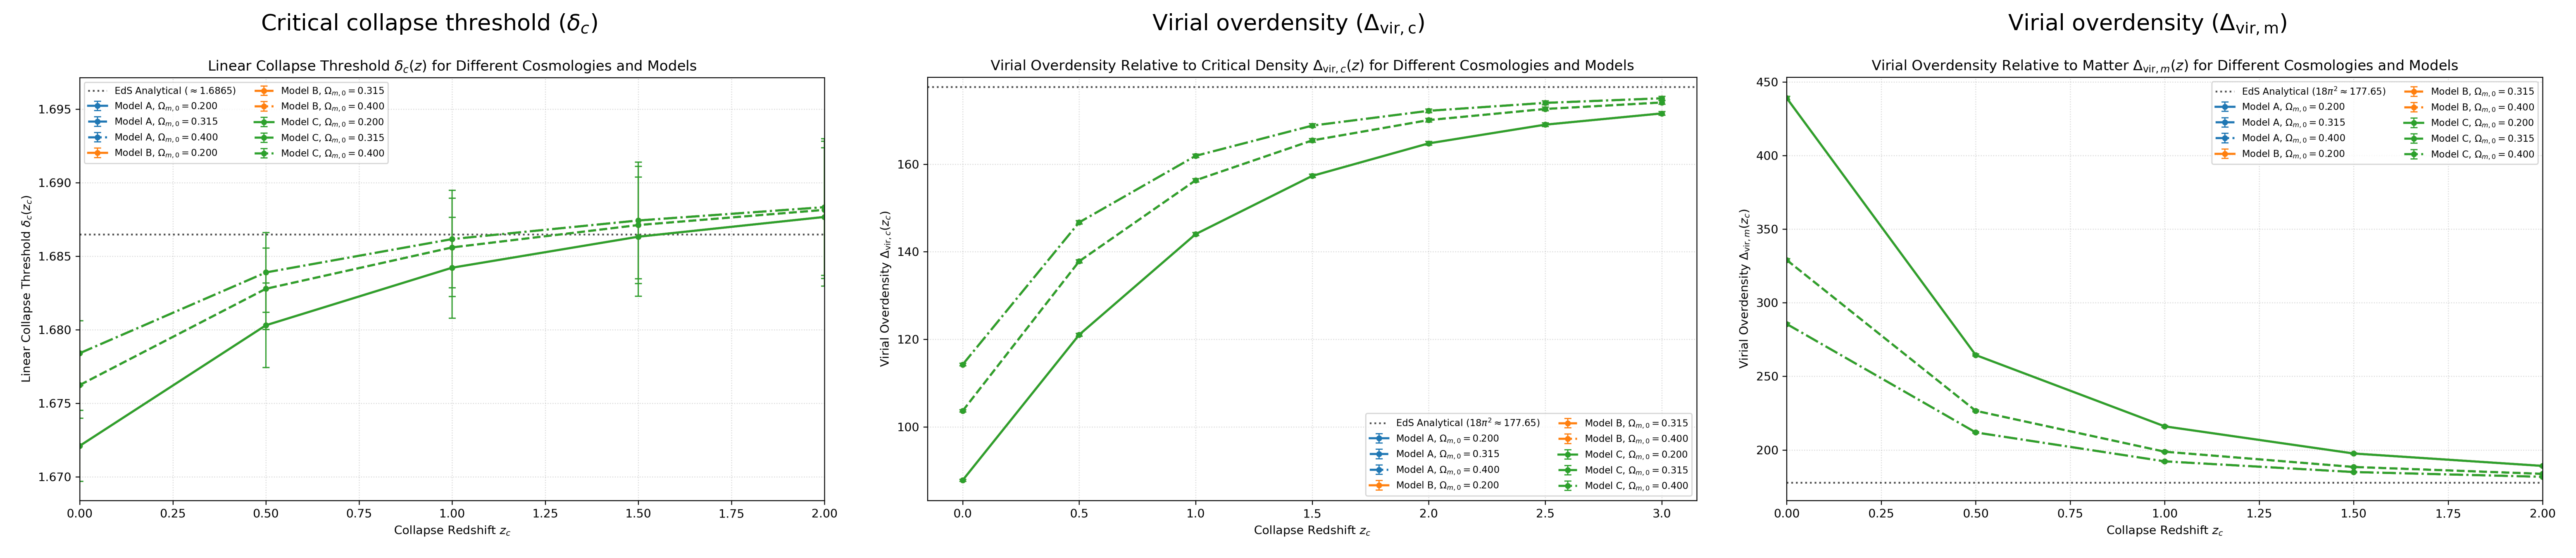
\includegraphics[width=\textwidth]{New_Figures/Test_20261020_154433_grid_observables.png}
        \caption{Spherical collapse observables $\delta_c(z_c)$ (left), $\Delta_{\mathrm{vir,m}}(z_c)$ (middle), and $\Delta_{\mathrm{vir,c}}(z_c)$ (right) computed across the 63-case cosmological grid for Models A, B, and C against Einstein--de Sitter reference values.}
        \label{fig:grid_observables}
    \end{figure}

The diagnostic verification checklist confirmed that varous cases were populated with finite values. The single check flagged as \texttt{False} during initial script execution was identified as a column key string mismatch (\texttt{y\_root\_poly} vs. \texttt{y\_root\_polynomial}); the physical root $y_{\mathrm{root\_poly}}$ matched $y_{\mathrm{vir}}$ identically across all 63 grid points.

\subsubsection{Convergence and Sensitivity Analysis}

Numerical convergence tests were performed in Einstein--de Sitter (EdS) and flat $\Lambda$CDM backgrounds by systematically varying
    \begin{enumerate}
        
        \item Initial scale factor $a_i \in \{10^{-3}, 10^{-4}, 10^{-5}\}$.
        
        \item Singular cutoff threshold $\delta_{\mathrm{stop}} \in \{10^5, 10^6, 10^7, 10^8\}$.
        
        \item Integration solver tolerances $(\mathrm{rtol}, \mathrm{atol}) \in \{(10^{-6}, 10^{-8}), (10^{-8}, 10^{-10}), (10^{-10}, 10^{-12})\}$.
        
    \end{enumerate}
    
    \begin{figure}[htbp]
        \centering
        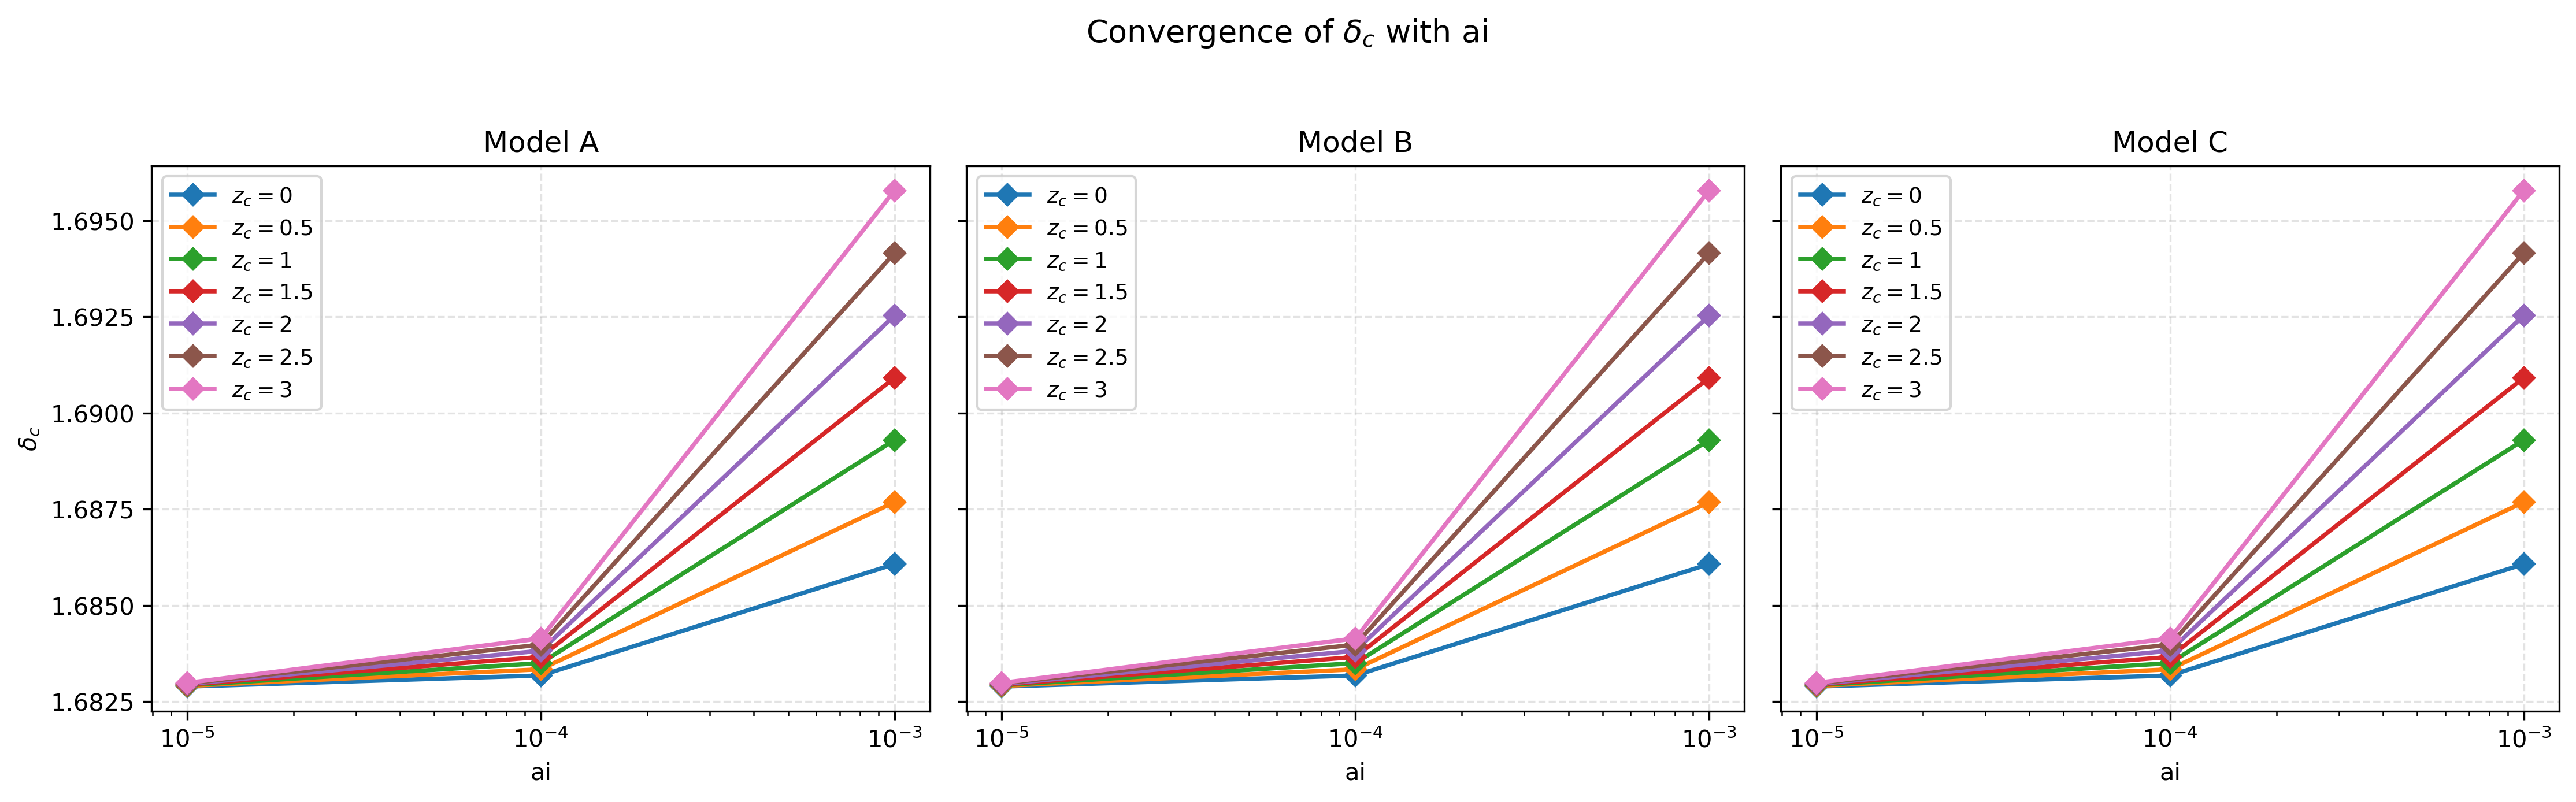
\includegraphics[width=0.95\textwidth]{New_Figures/Test_20261107_091134_convergence_delta_c_ai.png}
        \caption{Convergence of the linear collapse threshold $\delta_c$ with initial scale factor $a_i$ across Models A, B, and C.}
        \label{fig:conv_deltac_ai}
    \end{figure}
    
    \begin{figure}[htbp]
        \centering
        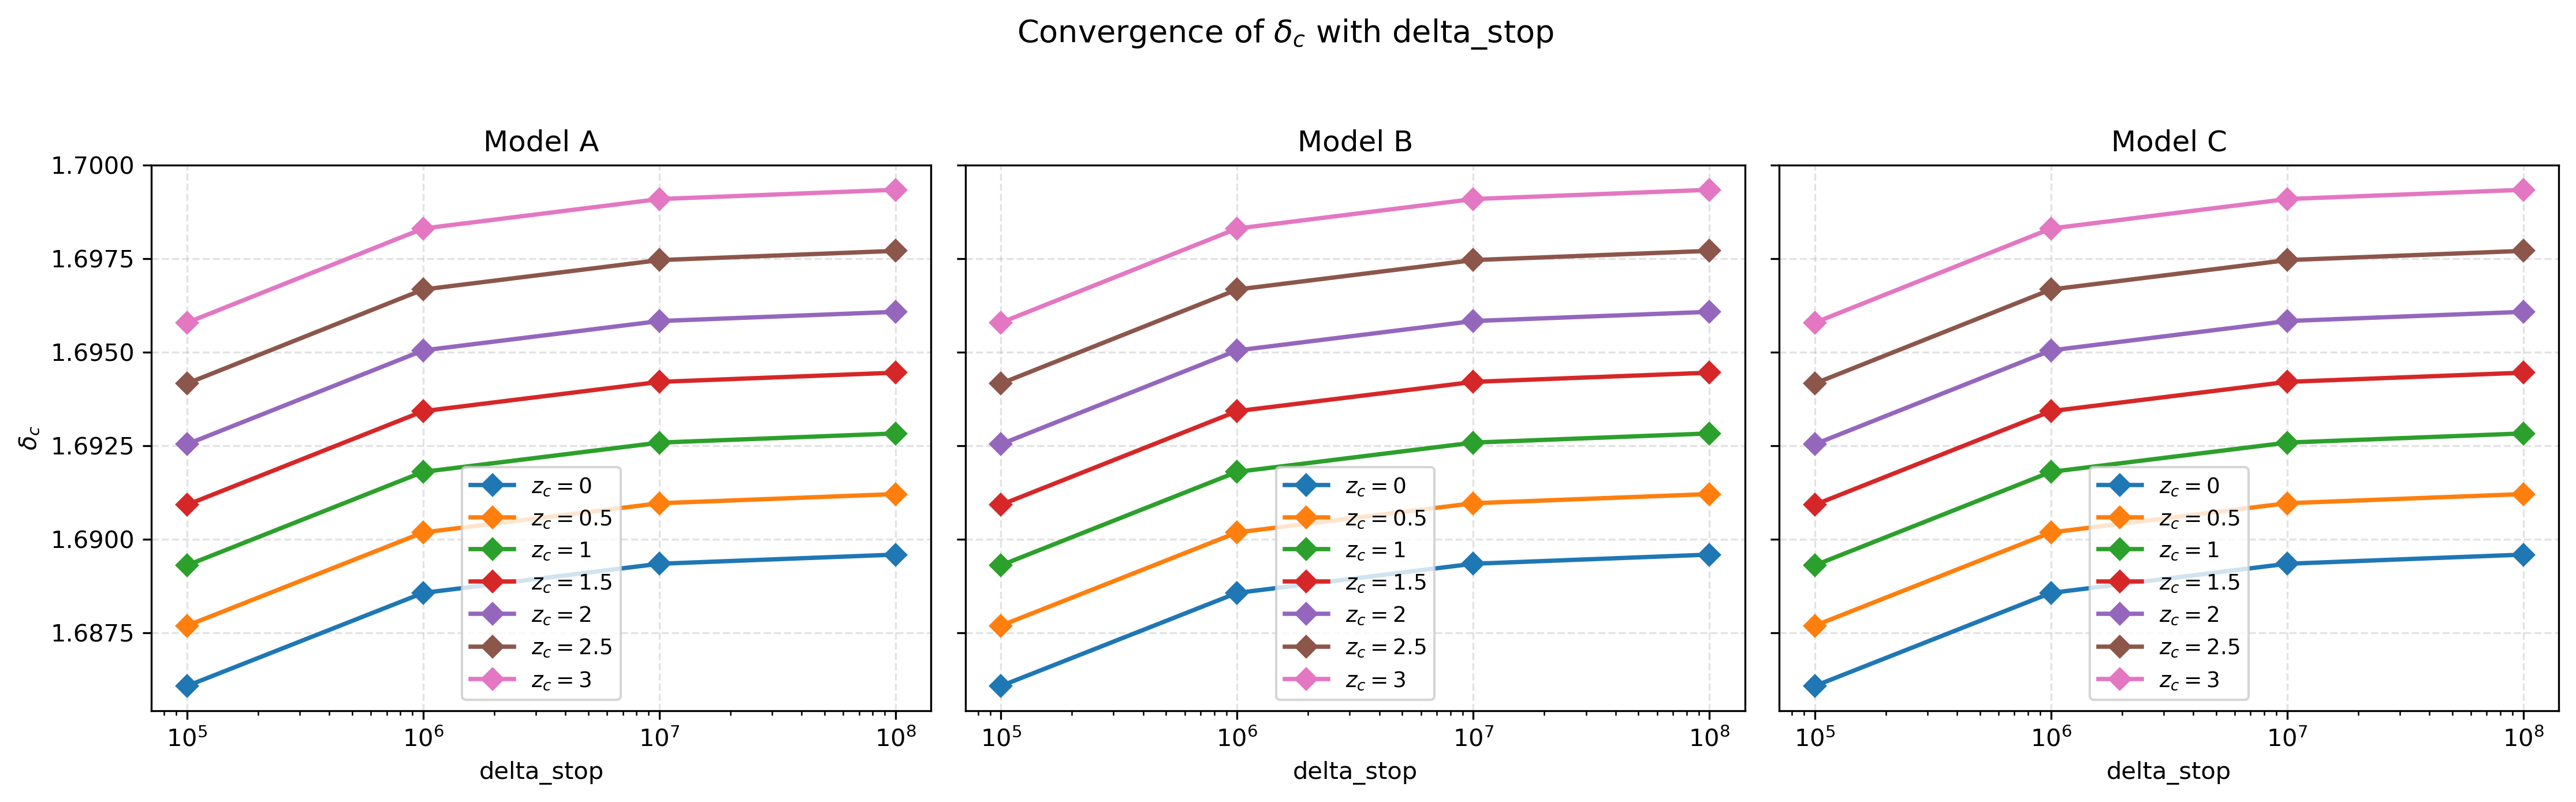
\includegraphics[width=\textwidth]{New_Figures/Test_20261107_091134_convergence_delta_c_delta_stop.png}
        \caption{Convergence of $\delta_c$ with singular threshold cutoff $\delta_{\mathrm{stop}}$.}
        \label{fig:conv_deltac_deltastop}
    \end{figure}
    
    \begin{figure}[htbp]
        \centering
        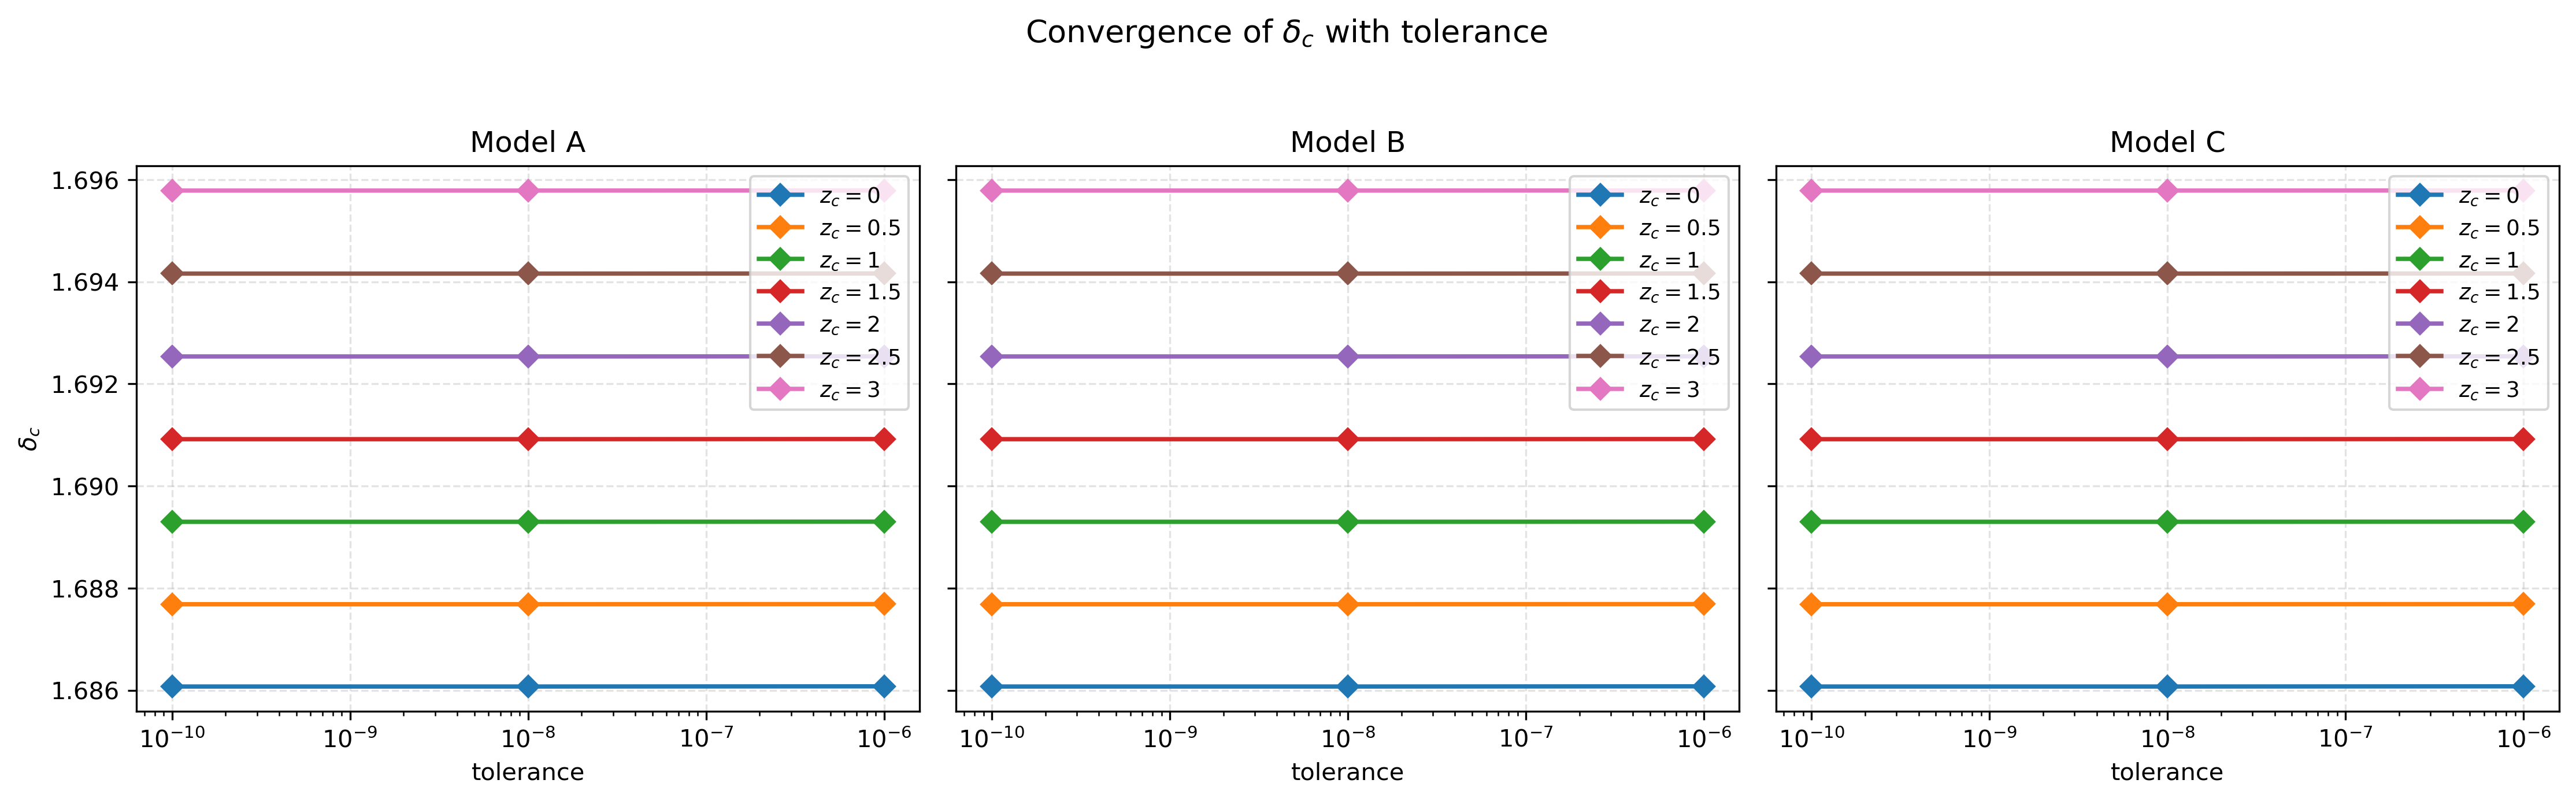
\includegraphics[width=\textwidth]{New_Figures/Test_20261107_091134_convergence_delta_c_tolerance.png}
        \caption{Dependence of $\delta_c$ on ODE integrator numerical tolerances.}
        \label{fig:conv_deltac_tol}
    \end{figure}
    
    \begin{figure}[htbp]
        \centering
        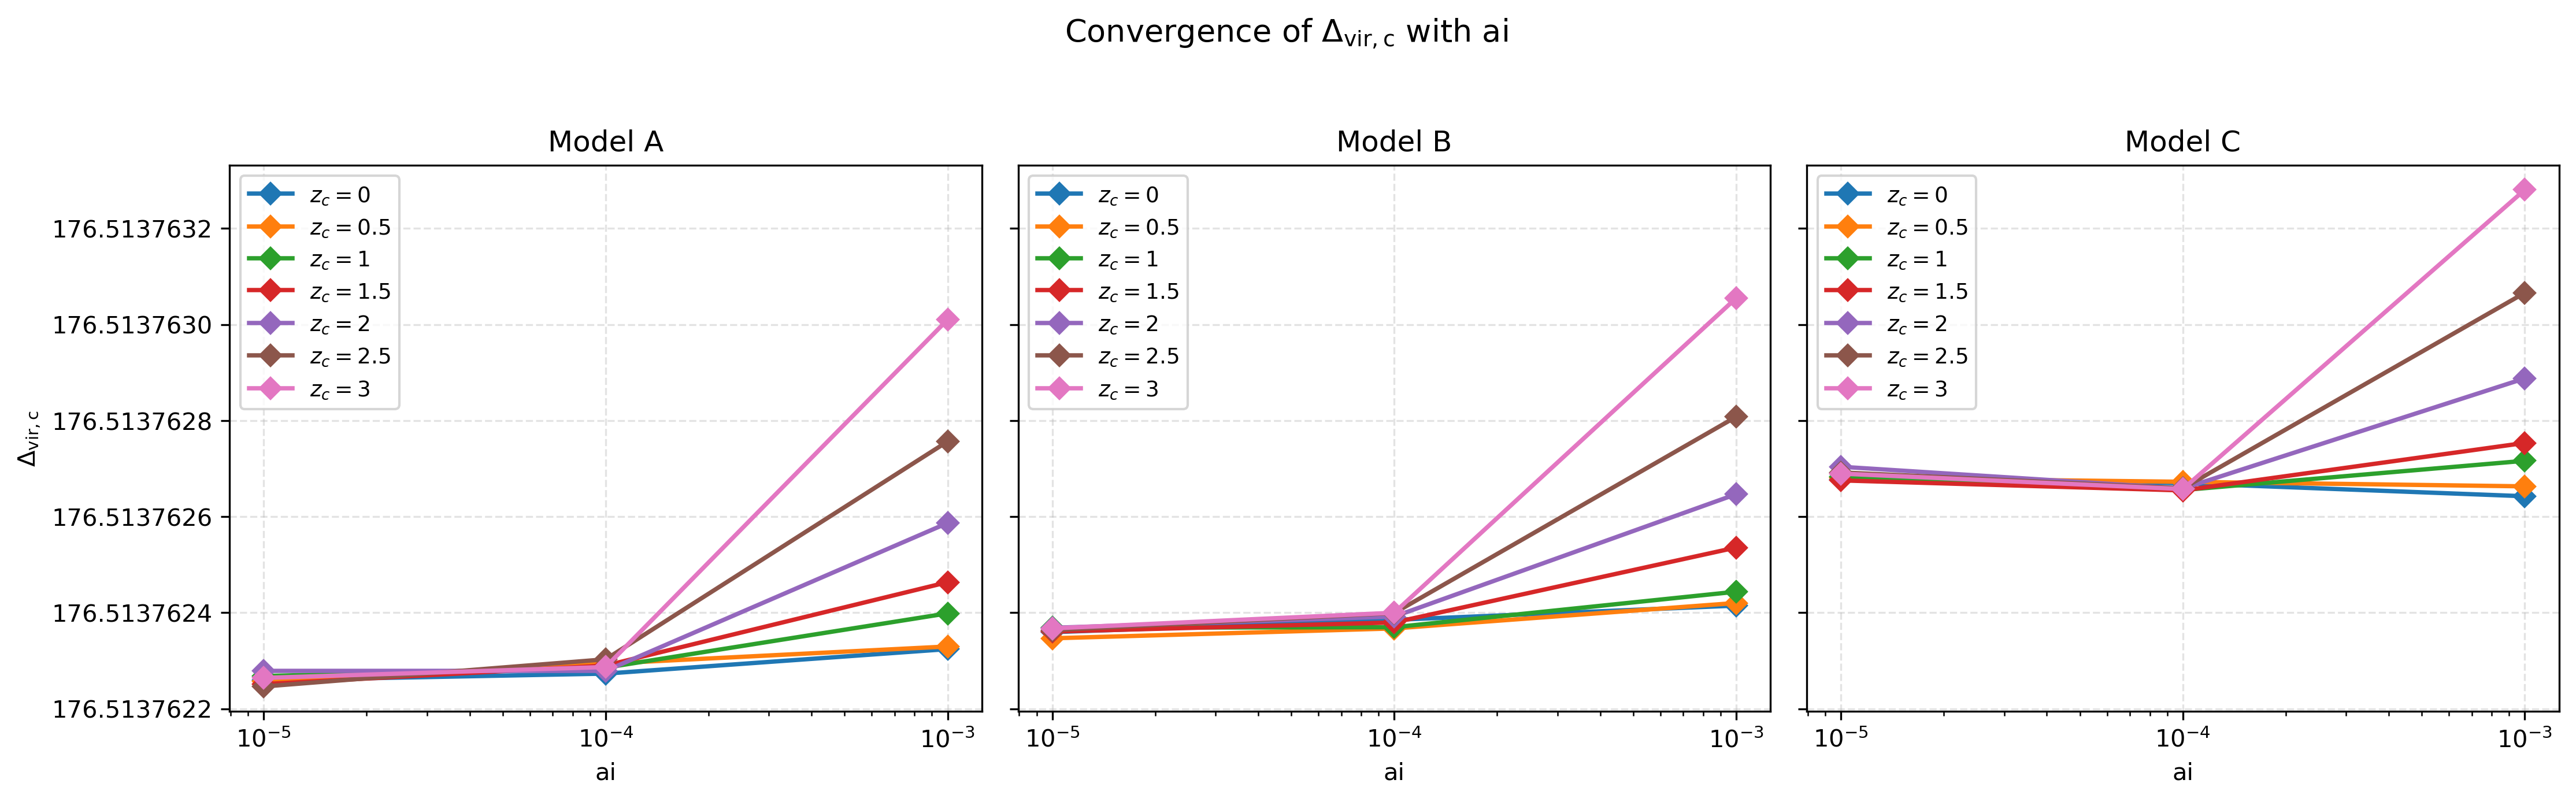
\includegraphics[width=\textwidth]{New_Figures/Test_20261107_091134_convergence_Delta_vir_c_ai.png}
        \caption{Convergence of the critical virial overdensity $\Delta_{\mathrm{vir,c}}$ as a function of $a_i$.}
        \label{fig:conv_vir_c_ai}
    \end{figure}
    
    \begin{figure}[htbp]
        \centering
        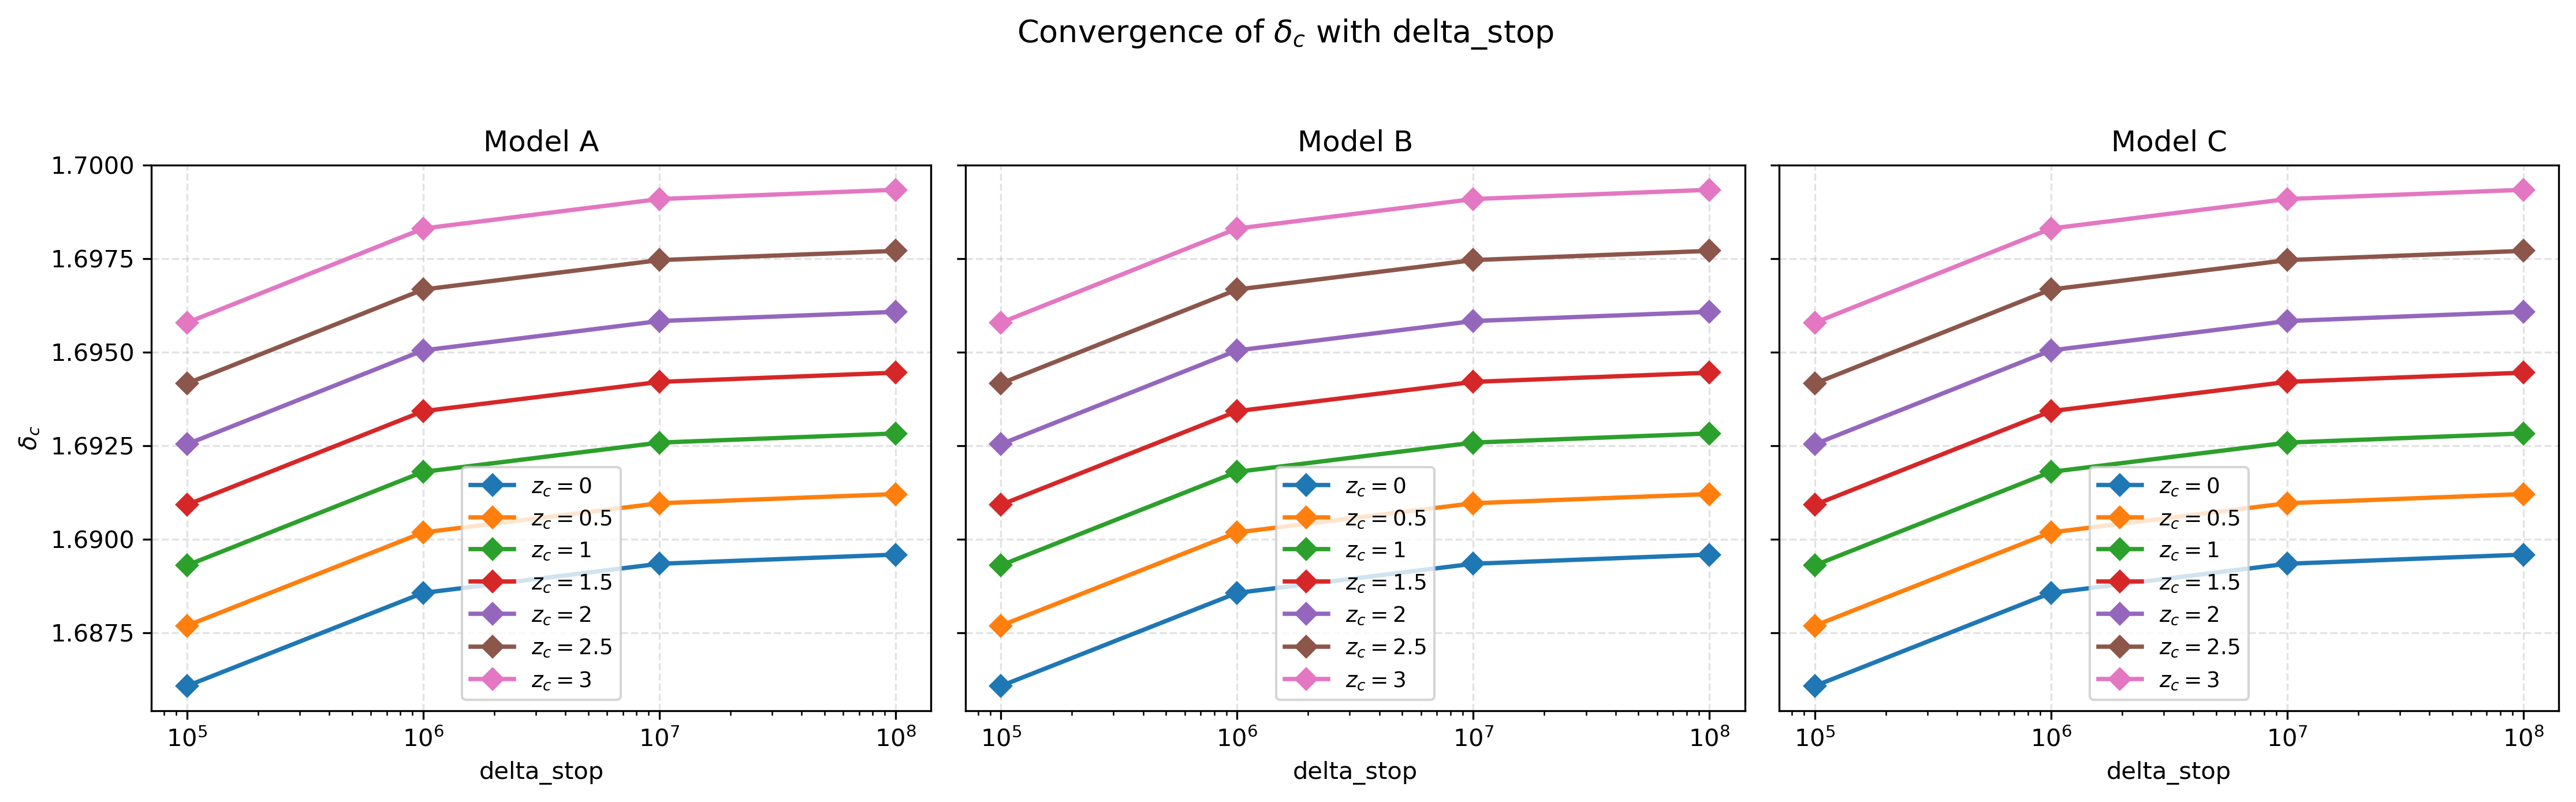
\includegraphics[width=\textwidth]{New_Figures/Test_20261107_091134_convergence_delta_c_delta_stop.png}
        \caption{Convergence of $\Delta_{\mathrm{vir,c}}$ with singular cutoff $\delta_{\mathrm{stop}}$.}
        \label{fig:conv_vir_c_deltastop}
    \end{figure}
    
    \begin{figure}[htbp]
        \centering
        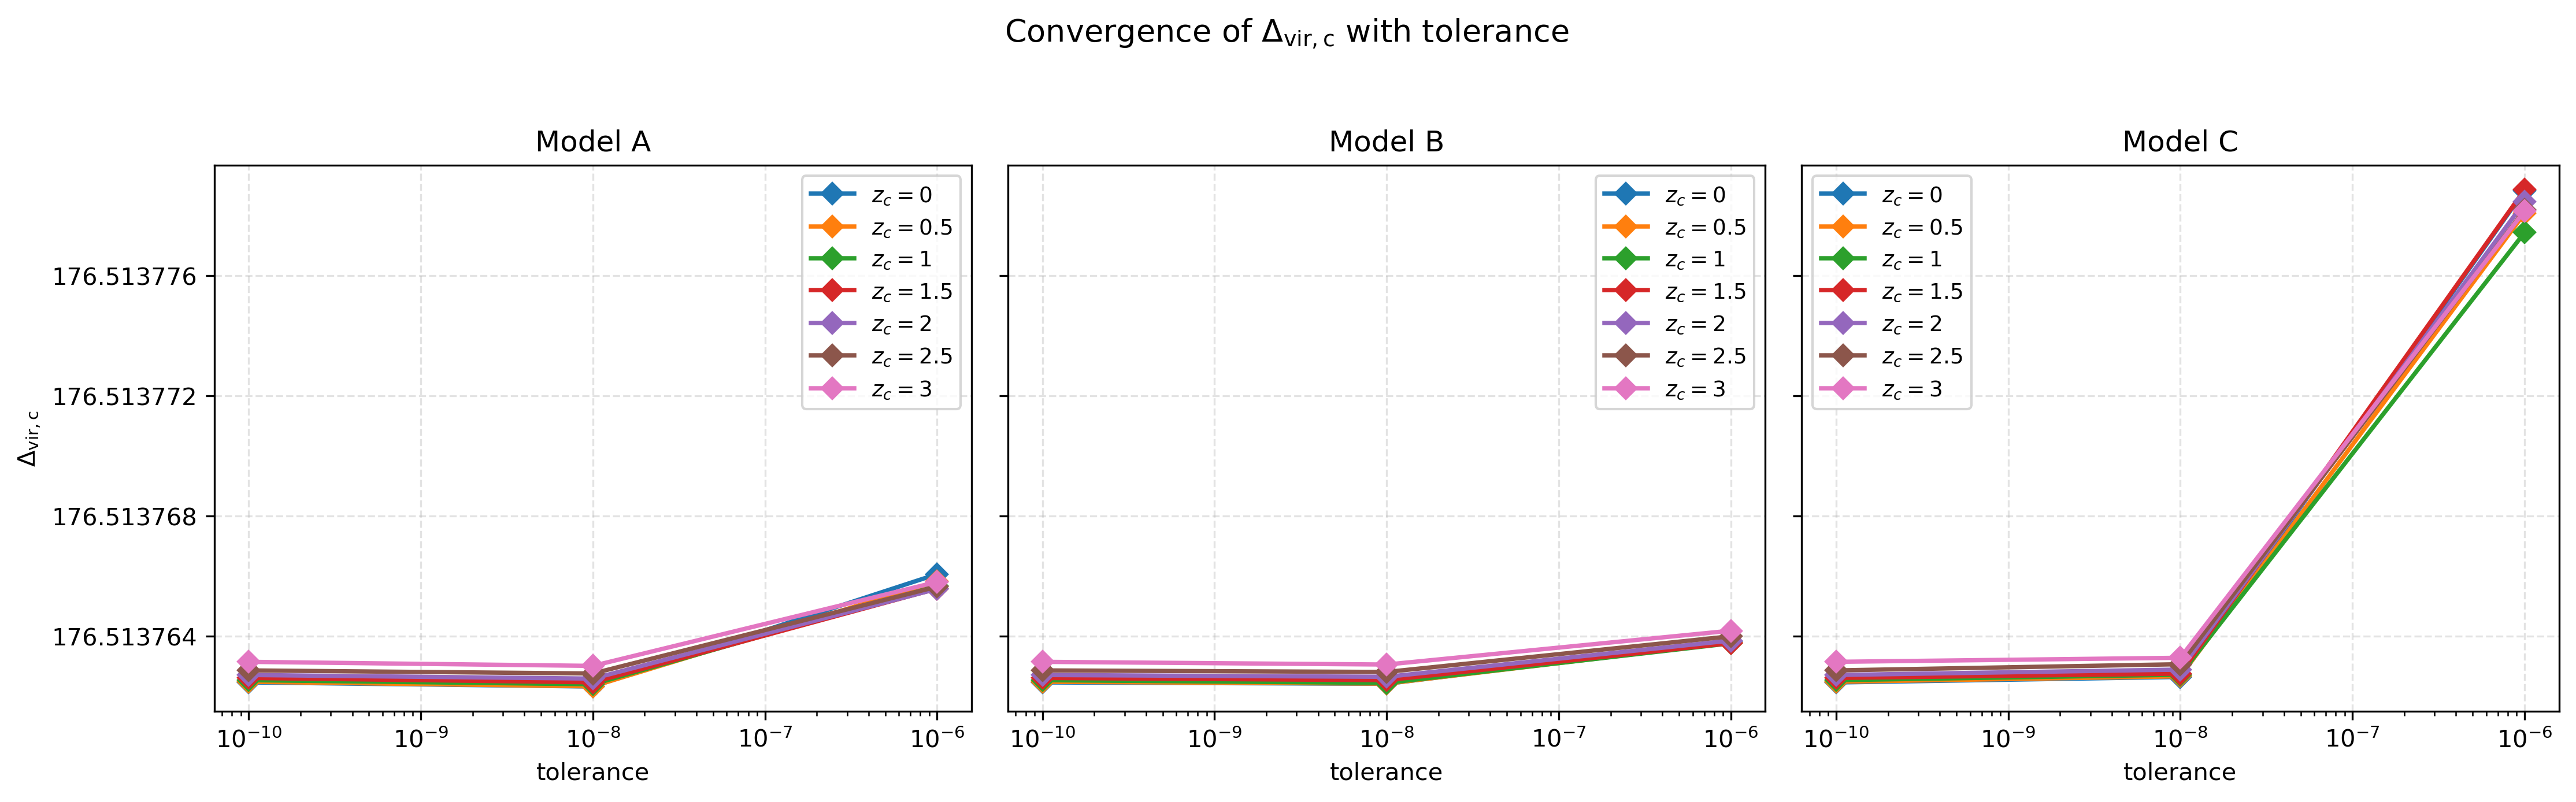
\includegraphics[width=\textwidth]{New_Figures/Test_20261107_091134_convergence_Delta_vir_c_tolerance.png}
        \caption{Dependence of $\Delta_{\mathrm{vir,c}}$ on solver integration tolerances.}
        \label{fig:conv_vir_c_tol}
    \end{figure}
    
    \begin{figure}[htbp]
        \centering
        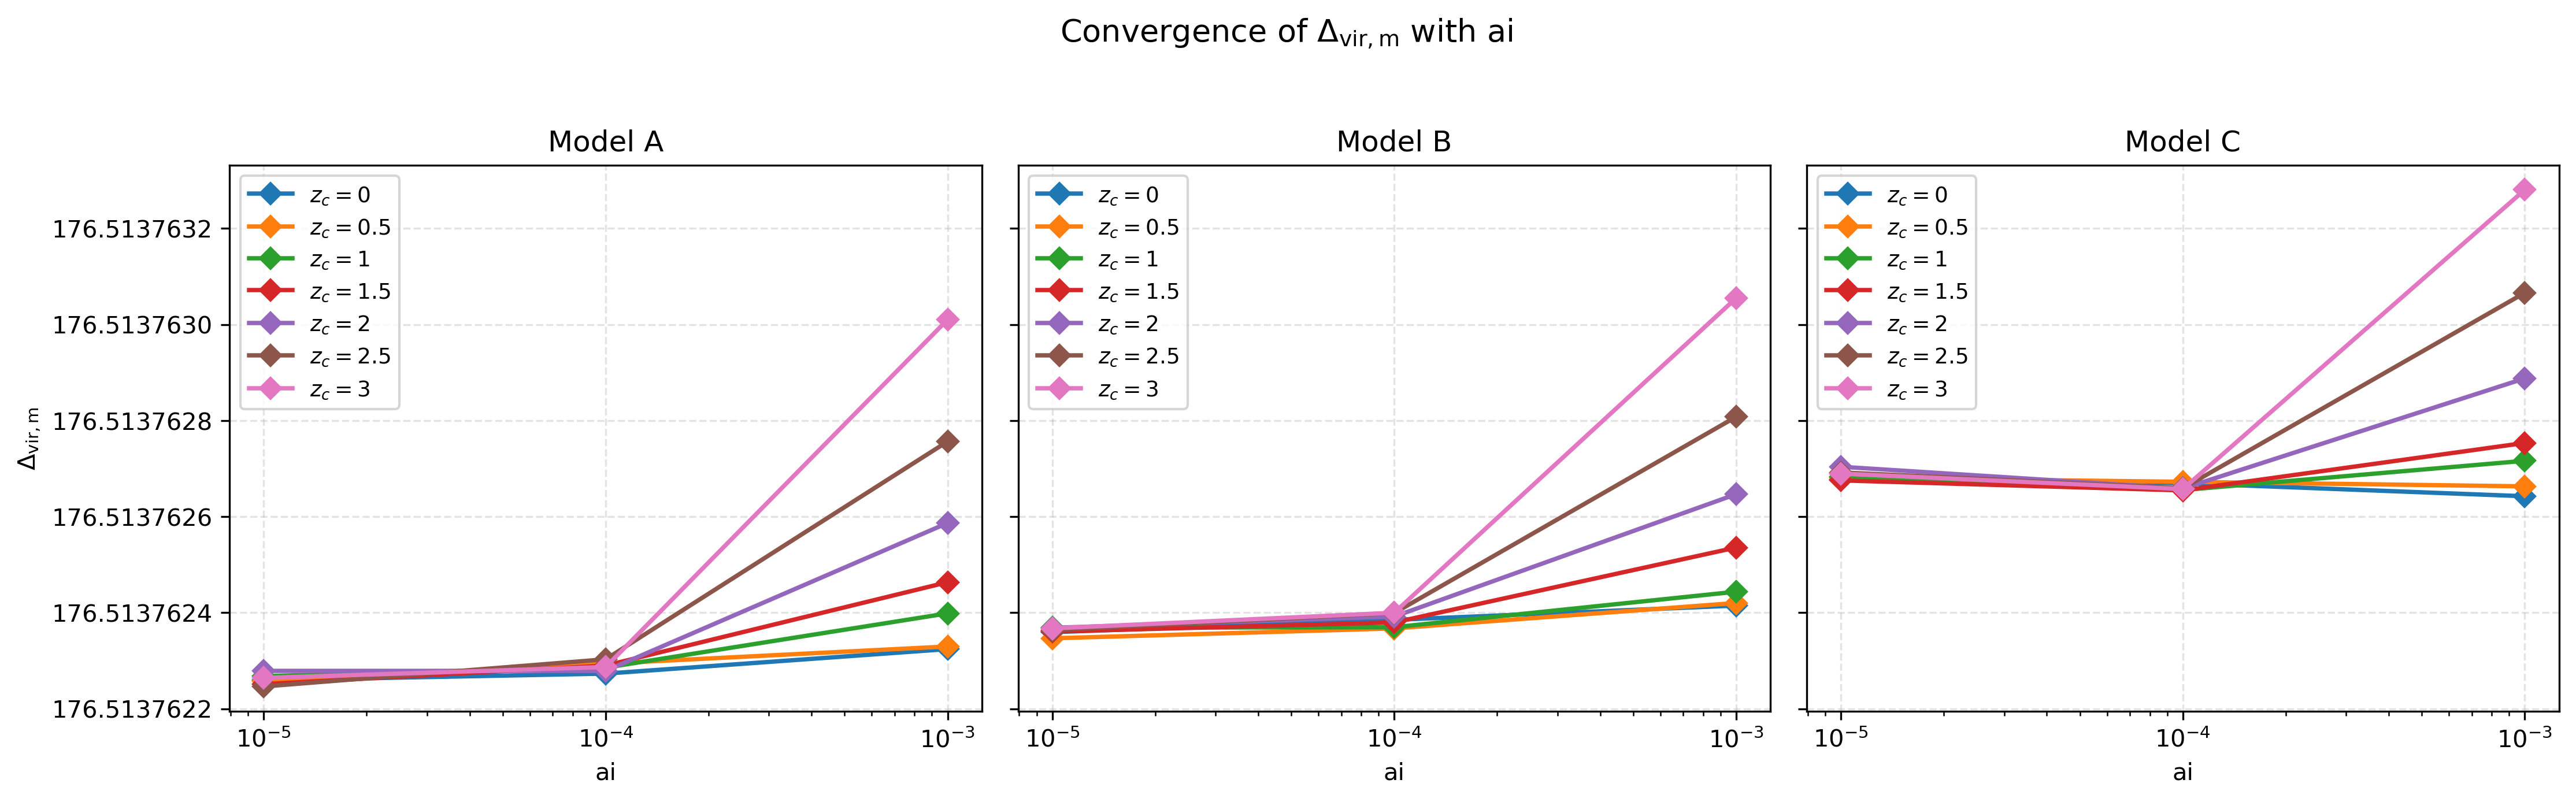
\includegraphics[width=\textwidth]{New_Figures/Test_20261107_091134_convergence_Delta_vir_m_ai.png}
        \caption{Convergence of the matter virial overdensity $\Delta_{\mathrm{vir,m}}$ as a function of $a_i$.}
        \label{fig:conv_vir_m_ai}
    \end{figure}
    
    \begin{figure}[htbp]
        \centering
        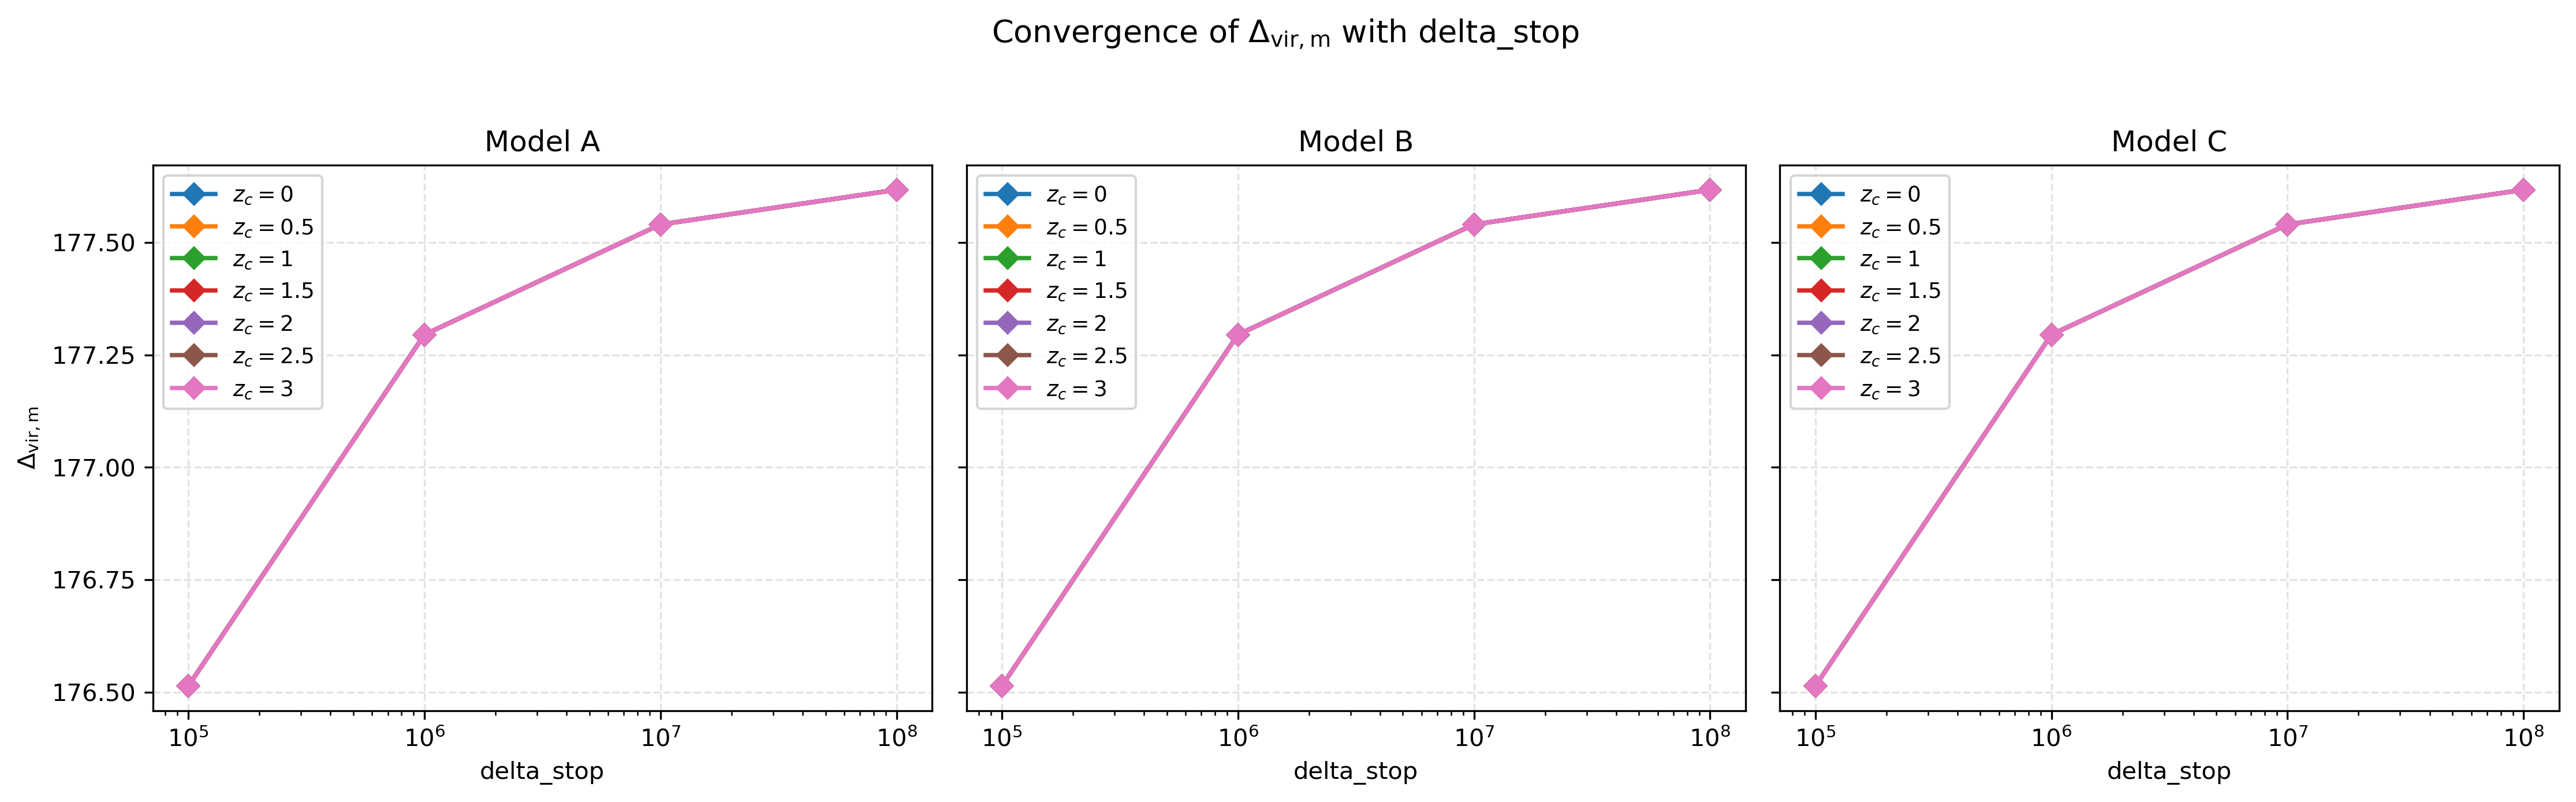
\includegraphics[width=\textwidth]{New_Figures/Test_20261107_091134_convergence_Delta_vir_m_delta_stop.png}
        \caption{Convergence of $\Delta_{\mathrm{vir,m}}$ with singular cutoff $\delta_{\mathrm{stop}}$.}
        \label{fig:conv_vir_m_deltastop}
    \end{figure}
    
    \begin{figure}[htbp]
        \centering
        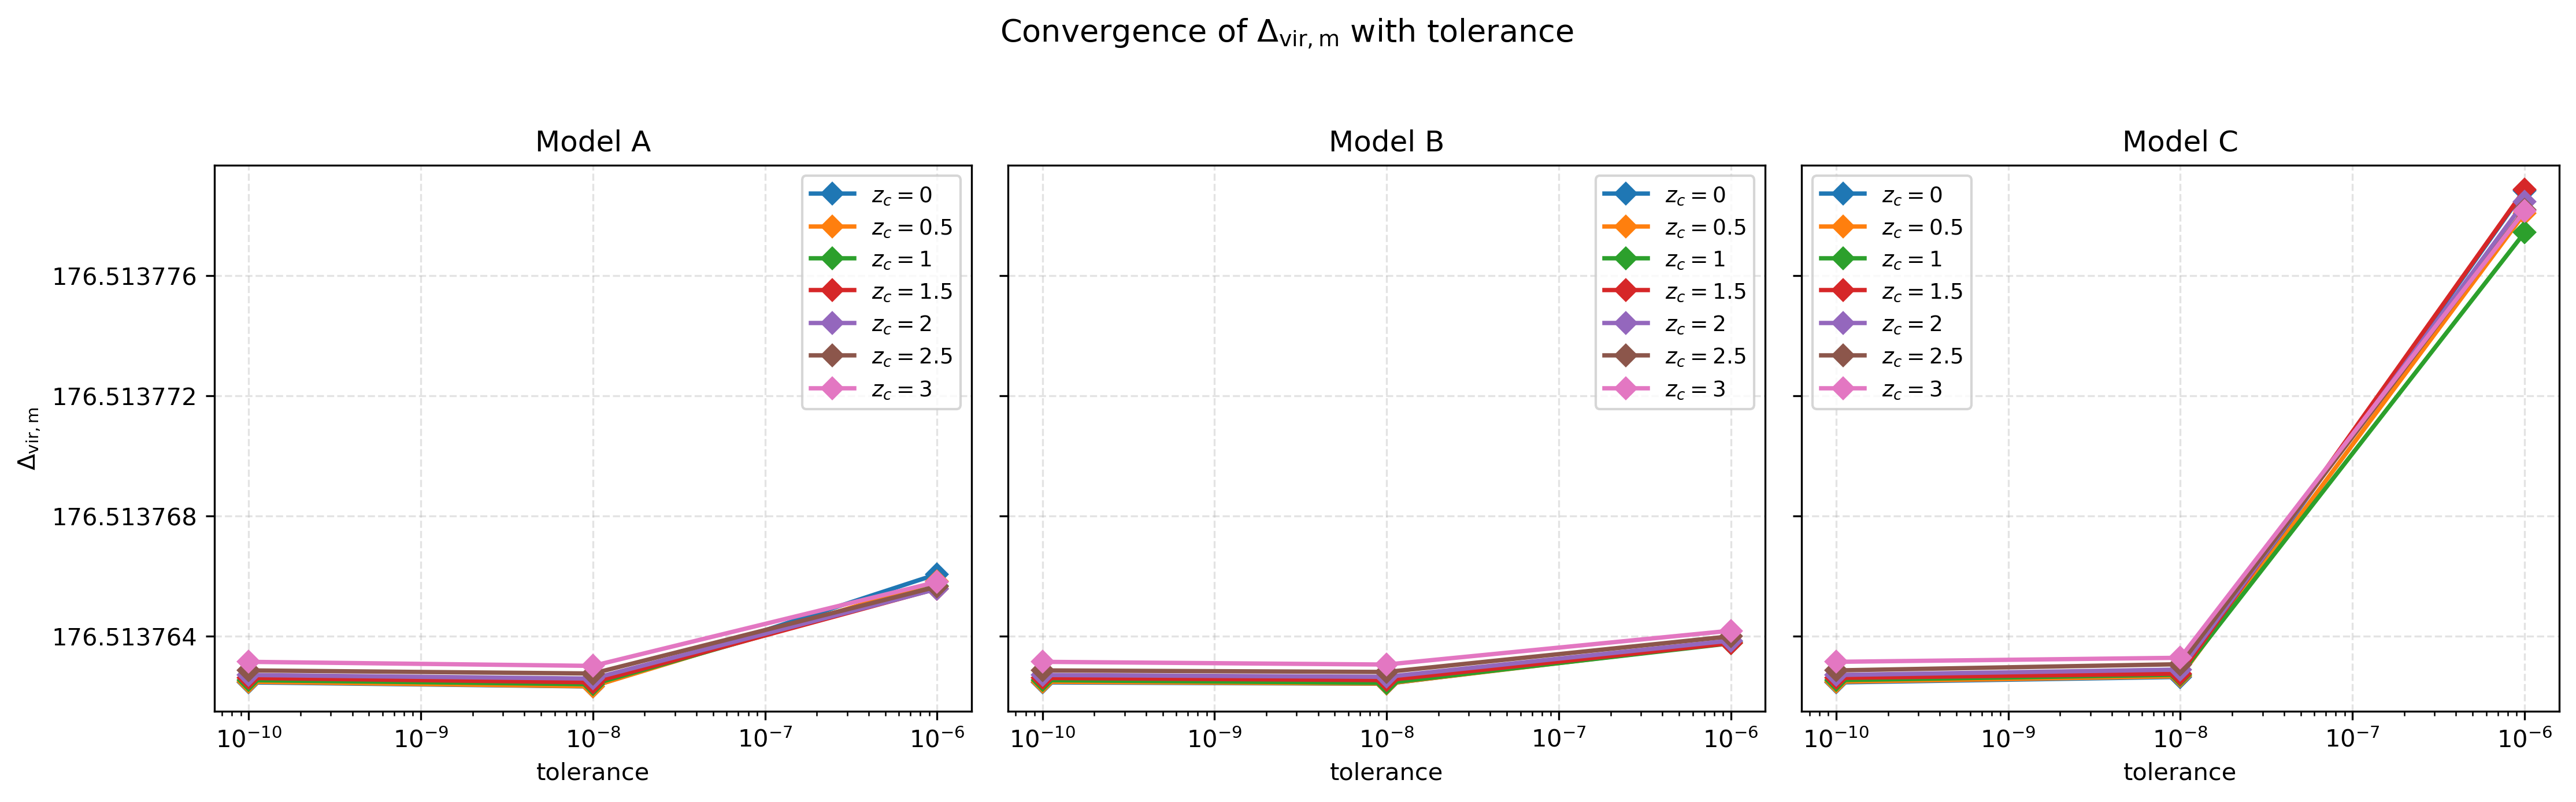
\includegraphics[width=\textwidth]{New_Figures/Test_20261107_091134_convergence_Delta_vir_m_tolerance.png}
        \caption{Dependence of $\Delta_{\mathrm{vir,m}}$ on solver integration tolerances.}
        \label{fig:conv_vir_m_tol}
    \end{figure}

The convergence study confirms that
    \begin{itemize}
    
        \item Transients from initial conditions decay rapidly for starting scale factors $a_i \le 10^{-4}$, where $\delta_c$ and virial overdensities stabilize.
        
        \item Increasing $\delta_{\mathrm{stop}} \ge 10^7$ ensures that the numerical cutoff converges to the true formal collapse singularity.
        
        \item Solver integration tolerances $(\mathrm{rtol}, \mathrm{atol}) \le (10^{-8}, 10^{-10})$ yield flat convergence profiles across all observables.
        
    \end{itemize}